\chapter{Исследовательская часть}

В данном разделе будут приведены примеры работы программы, и будет проведён сравнительный анализ реализованных алгоритмов сортировки по затраченному процессорному времени.


\section{Технические характеристики}

Проведем сравнительный анализ алгоритмов сортировки по затраченнному процессорному времени.

Тестирование проводилось на устройстве со следующими техническими характеристиками:

\begin{itemize}
	\item операционная система Windows 10 pro ;
	\item память 32 Гб;
	\item процессор 12th Gen Intel(R) Core(TM) i5-12400 2.50 ГГц.
\end{itemize}

Во время тестирования компьютер был нагружен только встроенными приложениями окружения, а также непосредственно системой тестирования.

\clearpage

\section{Демонстрация работы программы}

На рисунке \ref{img:example} приведен пример работы программы.

\begin{figure}[H]
	\begin{center}
		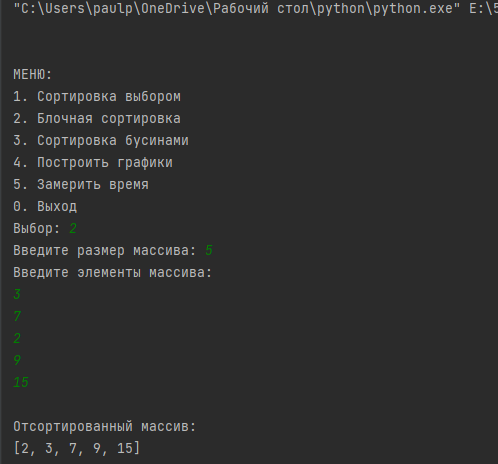
\includegraphics[scale=0.6]{img/example.png}
	\end{center}
	\captionsetup{justification=centering}
	\caption{Пример работы программы}
	\label{img:example}
\end{figure}

\section{Время выполнения алгоритмов}

Функция process\_time из библиотеки time языка программирования Python возвращает  процессорное время в секундах - значение типа float.

Для замера времени:
\begin{itemize}
	\item получить значение времени до начала сортировки, затем после её окончания. Чтобы получить результат, необходимо вычесть из второго значения первое;
	\item первый шаг необходимо повторить 500 раз, суммируя полученные значения, а затем усреднить результат.
\end{itemize}

Результаты замеров времени работы алгоритмов в миллисекундах приведены в таблицах \ref{tbl:best}, \ref{tbl:worst}, \ref{tbl:random}.

\begin{table}[h]
	\begin{center}
		\begin{threeparttable}
		\captionsetup{justification=raggedright,singlelinecheck=off}
		\caption{На входе отсортированный массив}
		\label{tbl:best}
		\begin{tabular}{|r|r|r|r|}
			\hline
			Размер & Выбором & Блочная & Бусинами \\
			\hline
  			 100 & 0.0938 & 0.0312 & 0.4062 \\ 
  			\hline
  			200 & 0.4062 & 0.0625 & 1.6875 \\ 
  			\hline
  			300 & 0.9375 & 0.1250 & 3.6875 \\ 
  			\hline
  			400 & 1.6562 & 0.2188 & 6.5625 \\ 
  			\hline
  			500 & 2.6562 & 0.2812 & 10.3438 \\ 
  			\hline
  			600 & 3.9062 & 0.3750 & 14.9062 \\ 
  			\hline
  			700 & 5.1562 & 0.4688 & 20.5000 \\ 
  			\hline
  			800 & 6.7812 & 0.5938 & 26.3750 \\ 
  			\hline
  			900 & 8.6875 & 0.7500 & 33.2812 \\ 
  			\hline
  			1000 & 10.7188 & 0.8750 & 41.2500 \\ 
  			\hline
		\end{tabular}
		\end{threeparttable}
    \end{center}
\end{table}

\begin{table}[h]
	\begin{center}
		\begin{threeparttable}
		\captionsetup{justification=raggedright,singlelinecheck=off}
		\caption{На входе отсортированный в обратном порядке массив}
		\label{tbl:worst}
		\begin{tabular}{|r|r|r|r|}
			\hline
			Размер & Выбором & Блочная & Бусинами \\
			\hline
  			  100 & 0.1250 & 0.0312 & 0.4375 \\ 
  			\hline
  			200 & 0.5312 & 0.0625 & 1.6875 \\ 
  			\hline
  			300 & 1.1250 & 0.1250 & 3.9375 \\ 
  			\hline
  			400 & 2.0625 & 0.1875 & 7.0312 \\ 
  			\hline
  			500 & 3.3438 & 0.2812 & 10.9688 \\ 
  			\hline
  			600 & 4.7500 & 0.3438 & 15.3438 \\ 
  			\hline
  			700 & 6.6562 & 0.4688 & 21.0000 \\ 
  			\hline
  			800 & 8.9062 & 0.5938 & 26.6250 \\ 
  			\hline
  			900 & 11.0000 & 0.7500 & 33.5312 \\ 
  			\hline
  			1000 & 13.6875 & 0.8750 & 42.1562 \\ 
  			\hline
  			
		\end{tabular}
		\end{threeparttable}
    \end{center}
\end{table}

\clearpage

\begin{table}[h]
	\begin{center}
		\begin{threeparttable}
		\captionsetup{justification=raggedright,singlelinecheck=off}
		\caption{На входе случайный массив}
		\label{tbl:random}
		\begin{tabular}{|r|r|r|r|}
			\hline
			Размер & Выбором & Блочная & Бусинами \\
			\hline
  			  100 & 0.1562 & 0.0312 & 8.0625 \\ 
  			\hline
  			200 & 0.4688 & 0.0625 & 16.8125 \\ 
  			\hline
  			300 & 0.9375 & 0.1875 & 24.5312 \\ 
  			\hline
  			400 & 1.6562 & 0.1875 & 33.0938 \\ 
  			\hline
  			500 & 2.7812 & 0.2188 & 41.2812 \\ 
  			\hline
  			600 & 4.0000 & 0.3438 & 49.9062 \\ 
  			\hline
  			700 & 5.5938 & 0.2500 & 57.9062 \\ 
  			\hline
  			800 & 7.7188 & 0.5625 & 66.3438 \\ 
  			\hline
  			900 & 8.7812 & 0.6875 & 75.3438 \\ 
  			\hline
  			1000 & 11.0312 & 0.9062 & 83.5625 \\ 
  			\hline
		\end{tabular}
		\end{threeparttable}
    \end{center}
\end{table}

На рисунках \ref{img:best-type}, \ref{img:worst-type}, \ref{img:random-type} приведены графические результаты замеров времени работы сортировок от длины входного массива в трех случаях: на входе отсортированный массив, отсортированный в обратном порядке и массив, заполненный случайным образом.

\begin{figure}[H]
	\begin{center}
		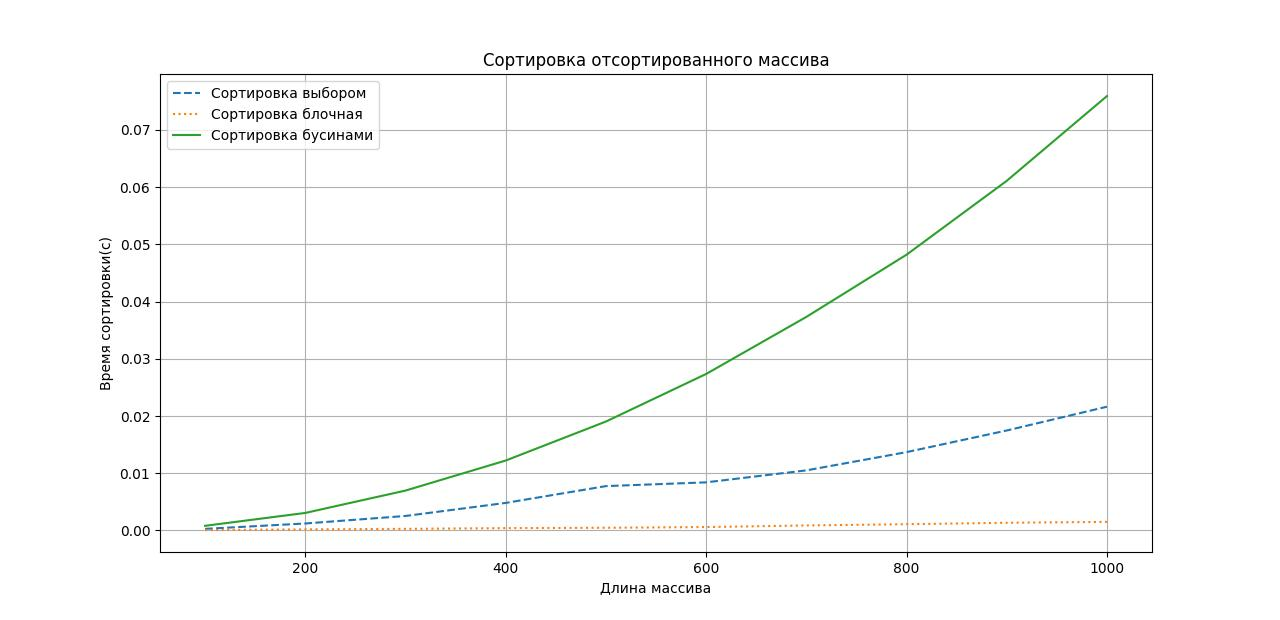
\includegraphics[scale=0.5]{img/best-type.jpg}
	\end{center}
	\captionsetup{justification=centering}
	\caption{На входе отсортированный массив}
	\label{img:best-type}
\end{figure}

\begin{figure}[H]
	\begin{center}
		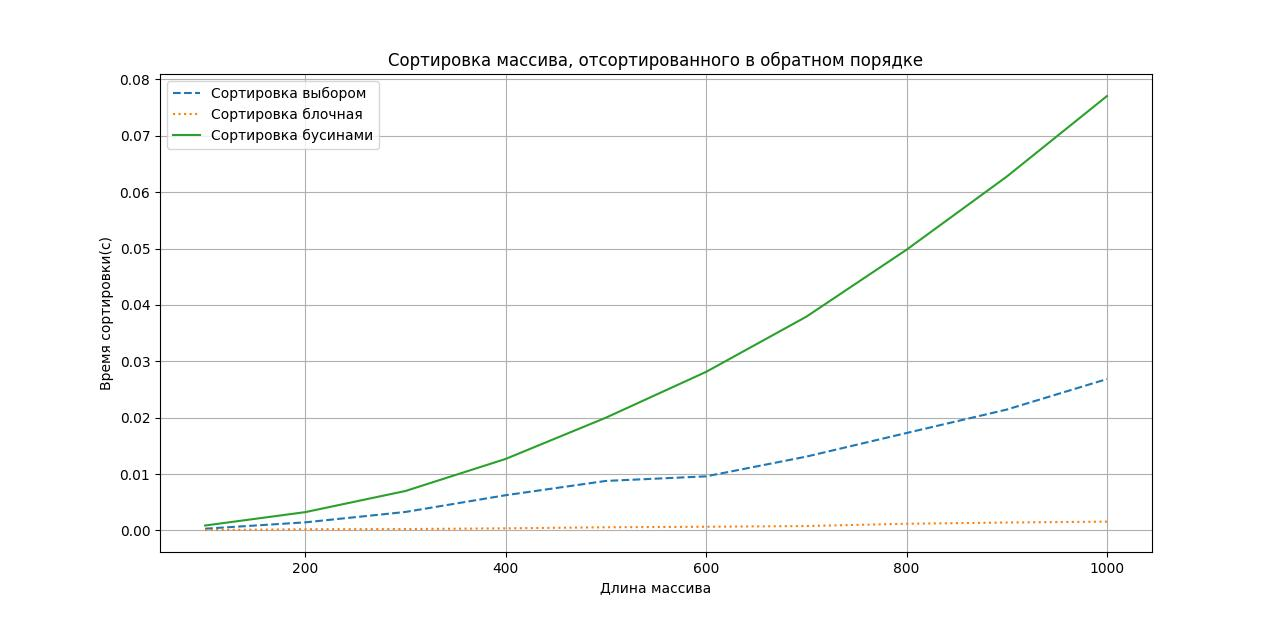
\includegraphics[scale=0.5]{img/worst-type.jpg}
	\end{center}
	\captionsetup{justification=centering}
	\caption{На входе отсортированный в обратном порядке массив}
	\label{img:worst-type}
\end{figure}

\begin{figure}[H]
	\begin{center}
		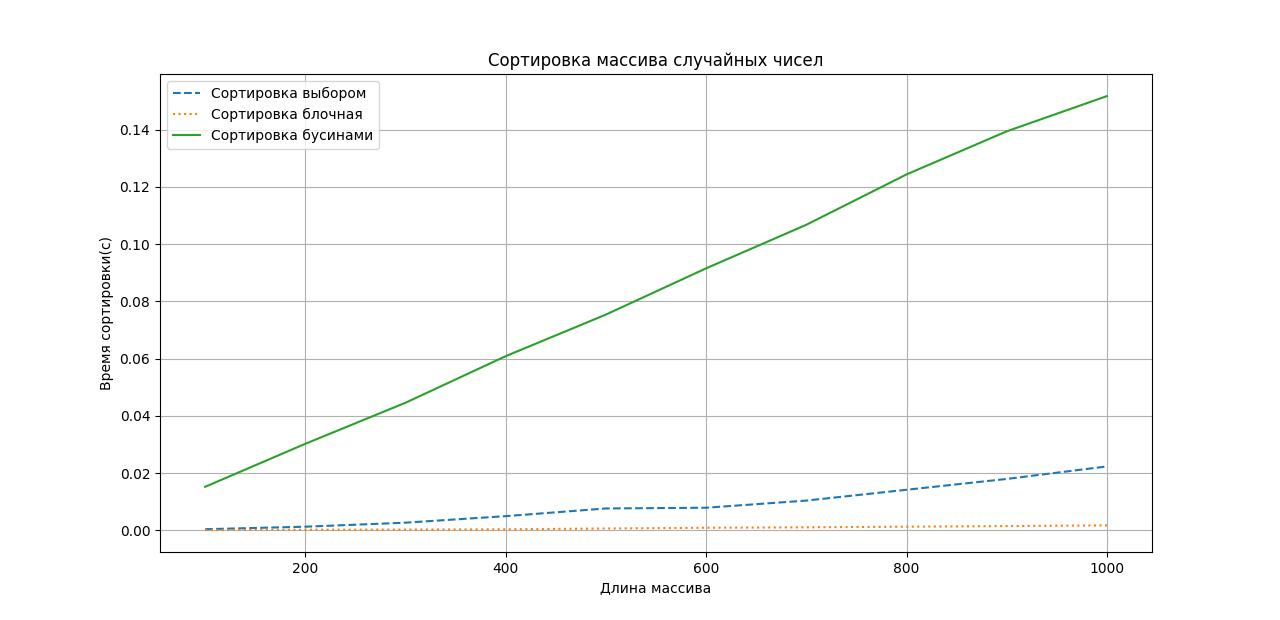
\includegraphics[scale=0.5]{img/random-type.jpg}
	\end{center}
	\captionsetup{justification=centering}
	\caption{На входе заполненный случайно массив}
	\label{img:random-type}
\end{figure}

\section*{Вывод}

Самой быстрой сортировкой из представленных является блочная сортировка. Затем по времени выполнения идет сортировка выбором. Самой же долгой сортировкой из представленных является сортировка бусинами.
